\cleardoublepage
{
\chapternonum{附录}

\appendixsecmajornumbering

\section{更多SCV检测算法的典型案例}
本部分内容是对第三章中SCV算法的检测性能检验部分的补充,参见正文\pageref{fig:detect_details}页相关内容。

\autoref{fig:detect_details2}给出了更多应用SCV算法进行波形检测的案例。可以看到,在大多数场景里SCV算法有着优异的检测性能,但对某些数据的检测处理仍有进一步提高的空间。
\begin{figure}[htbp]
    \centering
    \subfigure[\label{fig:c_by}被试BY的波形检测结果(局部)]{
    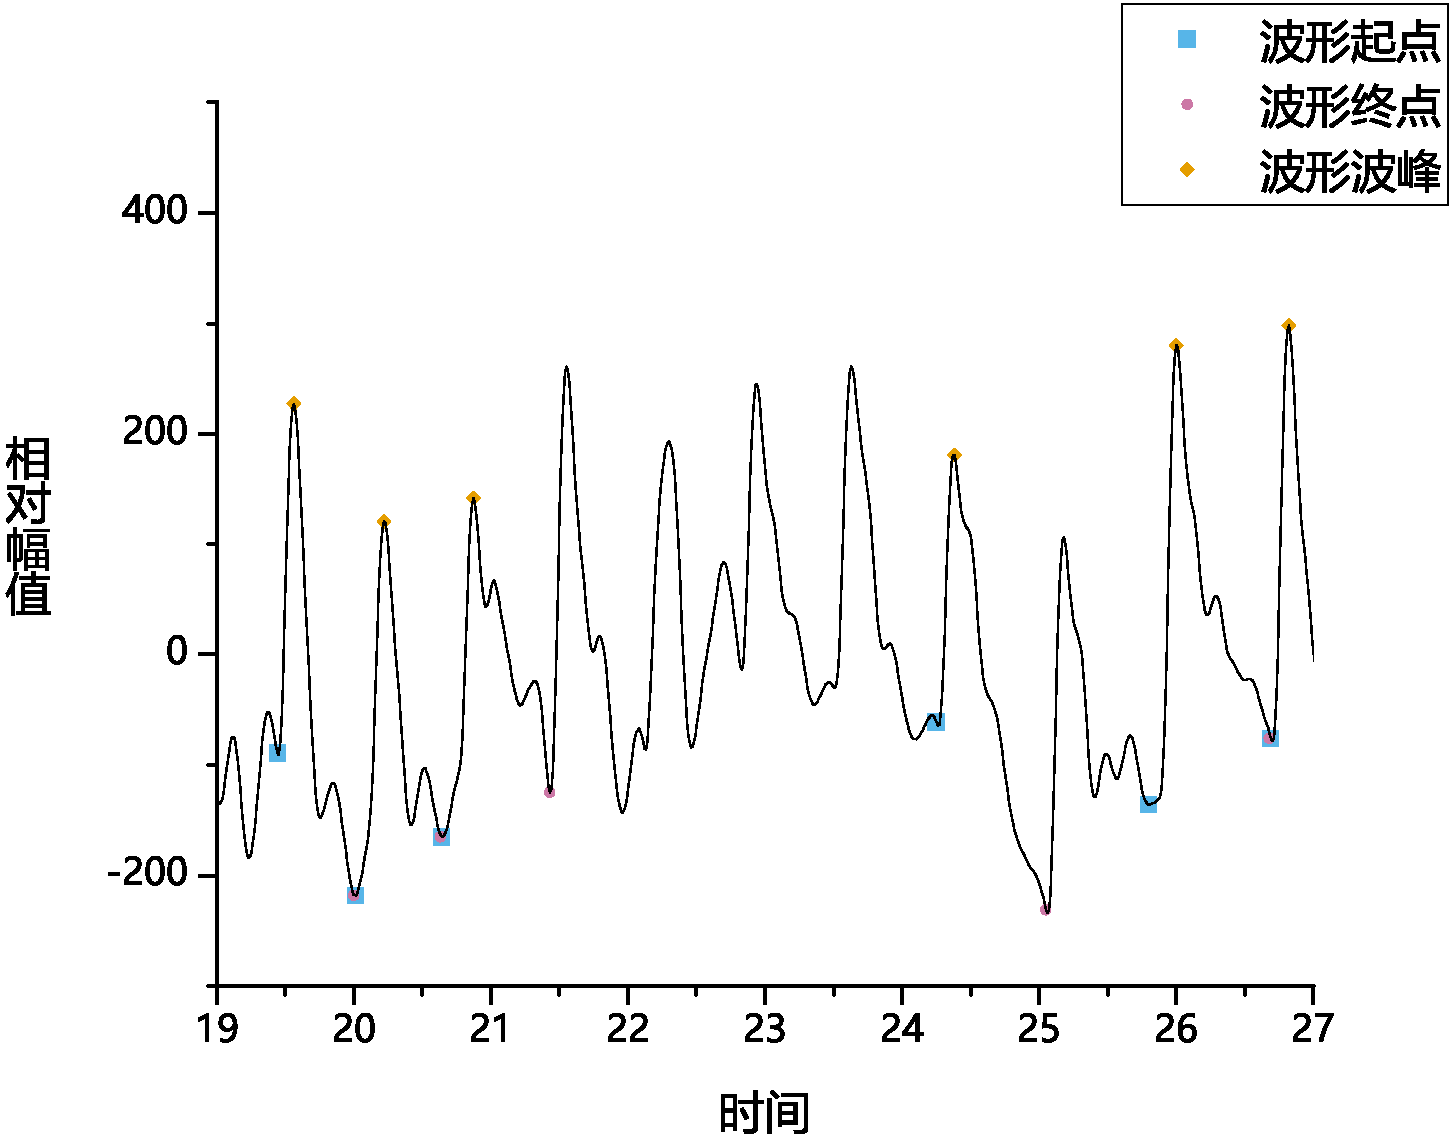
\includegraphics[width=7.5cm]{pulse_preprocess/check/by}
    }
    \quad
    \subfigure[\label{fig:c_ljj}被试LJJ的波形检测结果(局部)]{
    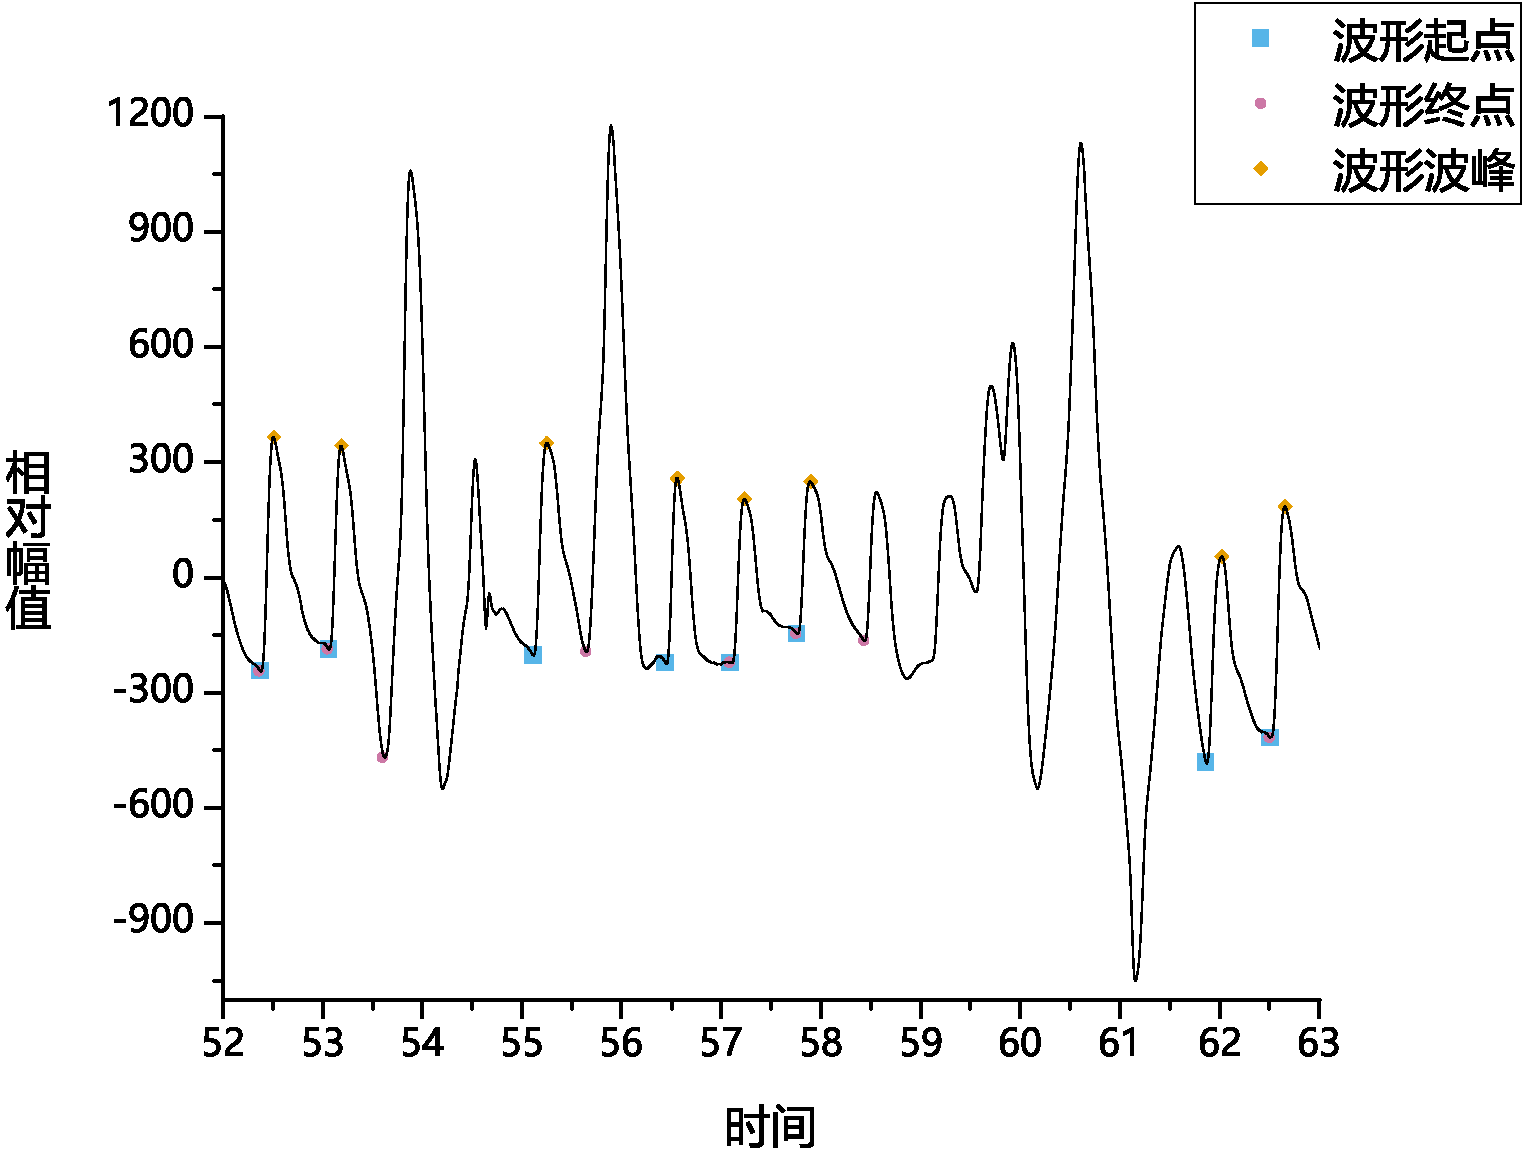
\includegraphics[width=7.5cm]{pulse_preprocess/check/ljj}
    }
    \quad
    \subfigure[\label{fig:c_rmq}被试RMQ的波形检测结果(局部)]{
        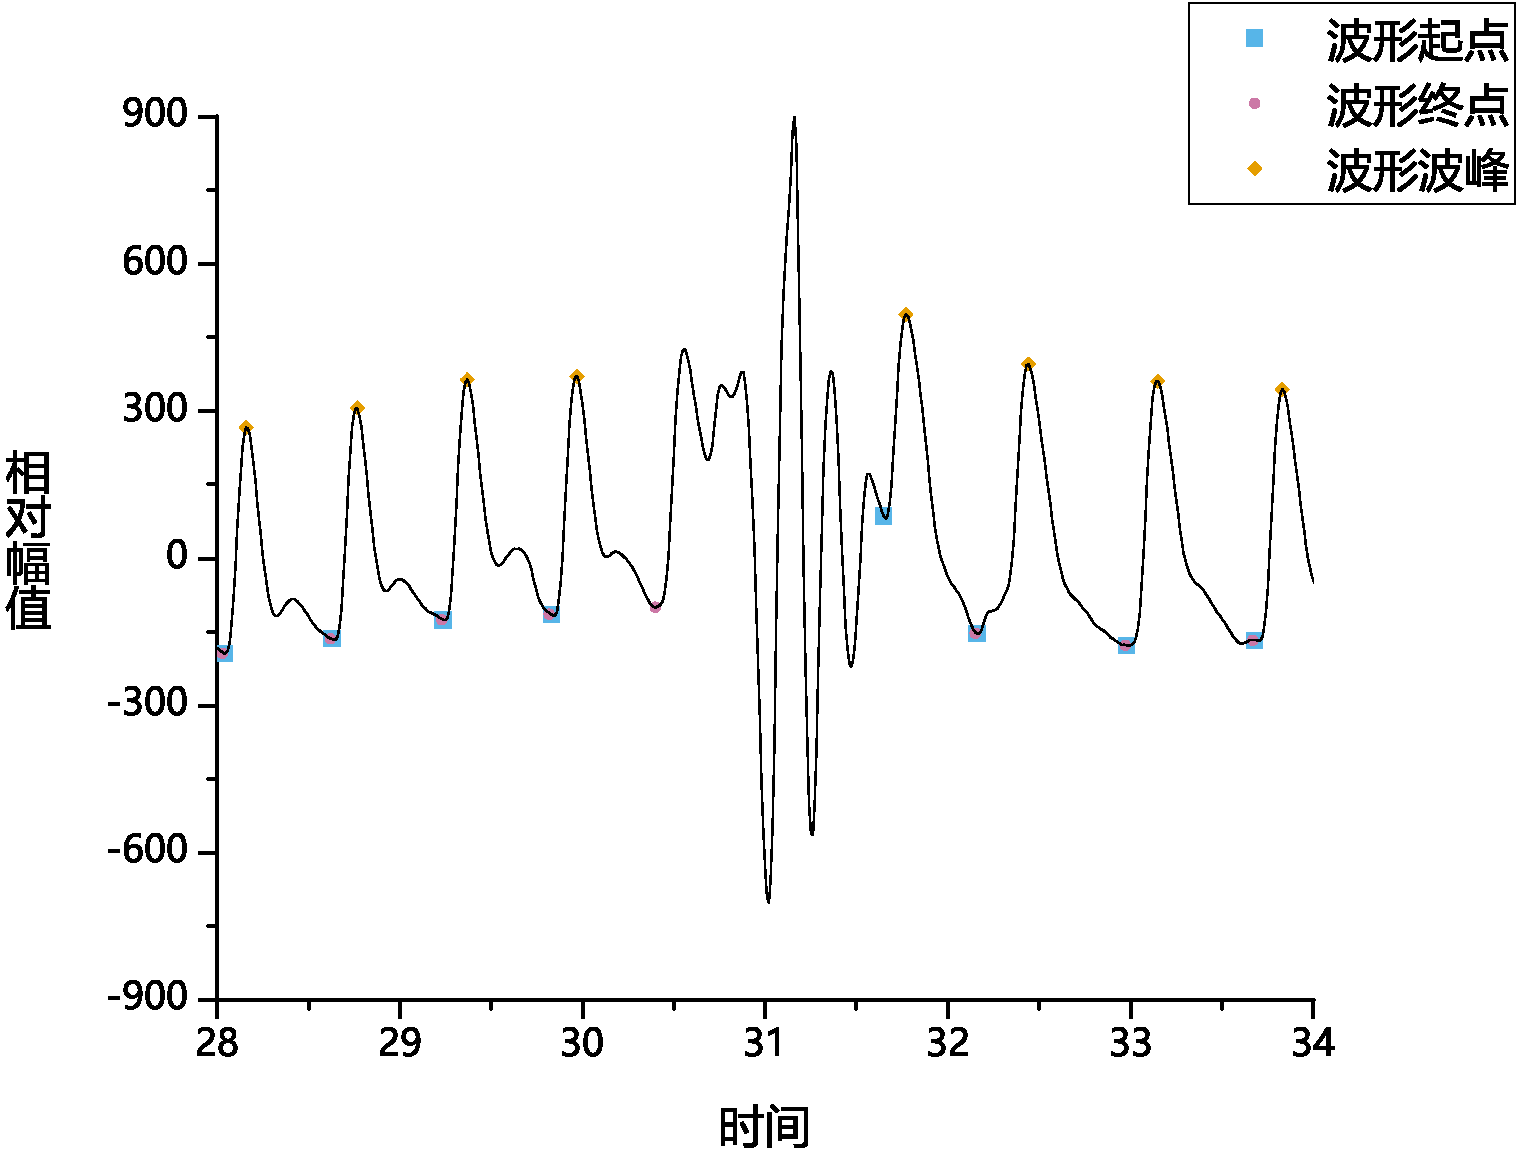
\includegraphics[width=7.5cm]{pulse_preprocess/check/rmq}
    }
    \quad
    \subfigure[\label{fig:c_wc}被试WC的波形检测结果(局部)]{
        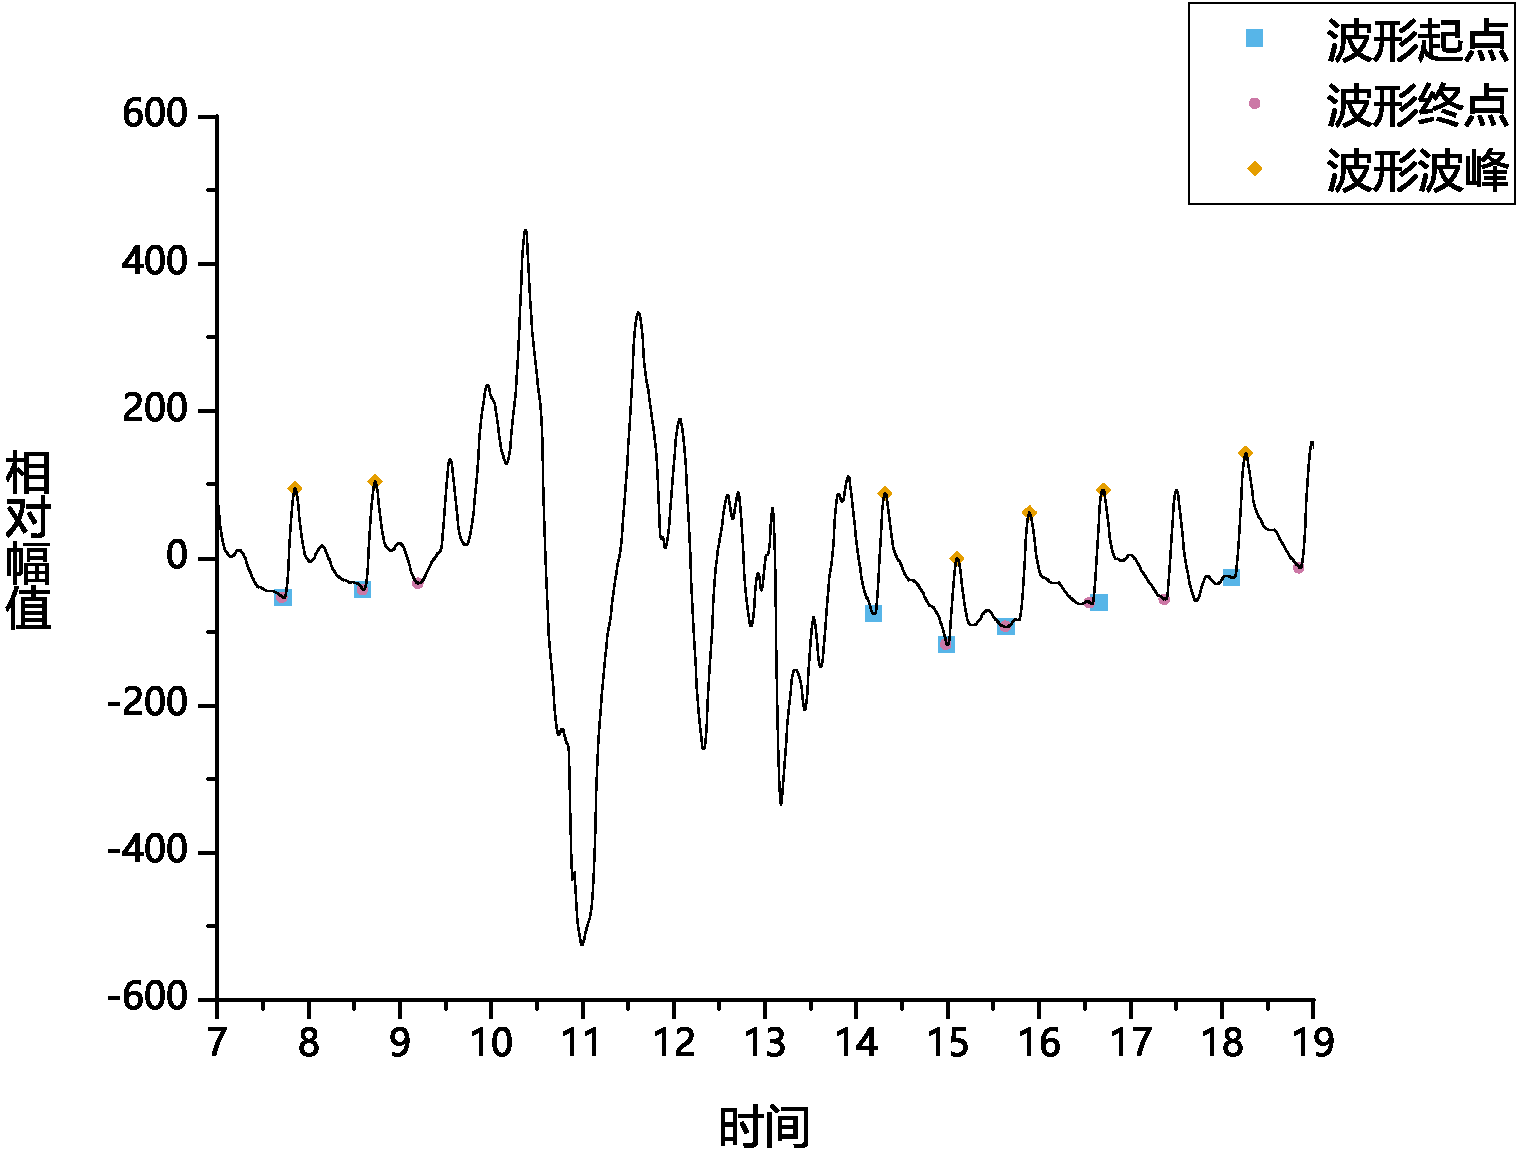
\includegraphics[width=7.5cm]{pulse_preprocess/check/wc2}
    }
    \caption{\label{fig:detect_details2}SCV算法对复杂信号的检测效果示意(补充)}
\end{figure}
\addtocounter{figure}{-1} % 将图的编号减1
\begin{figure}
\addtocounter{subfigure}{4} % 子图编号加4
    \quad
    \subfigure[\label{fig:c_why}被试WHY的波形检测结果(局部)]{
        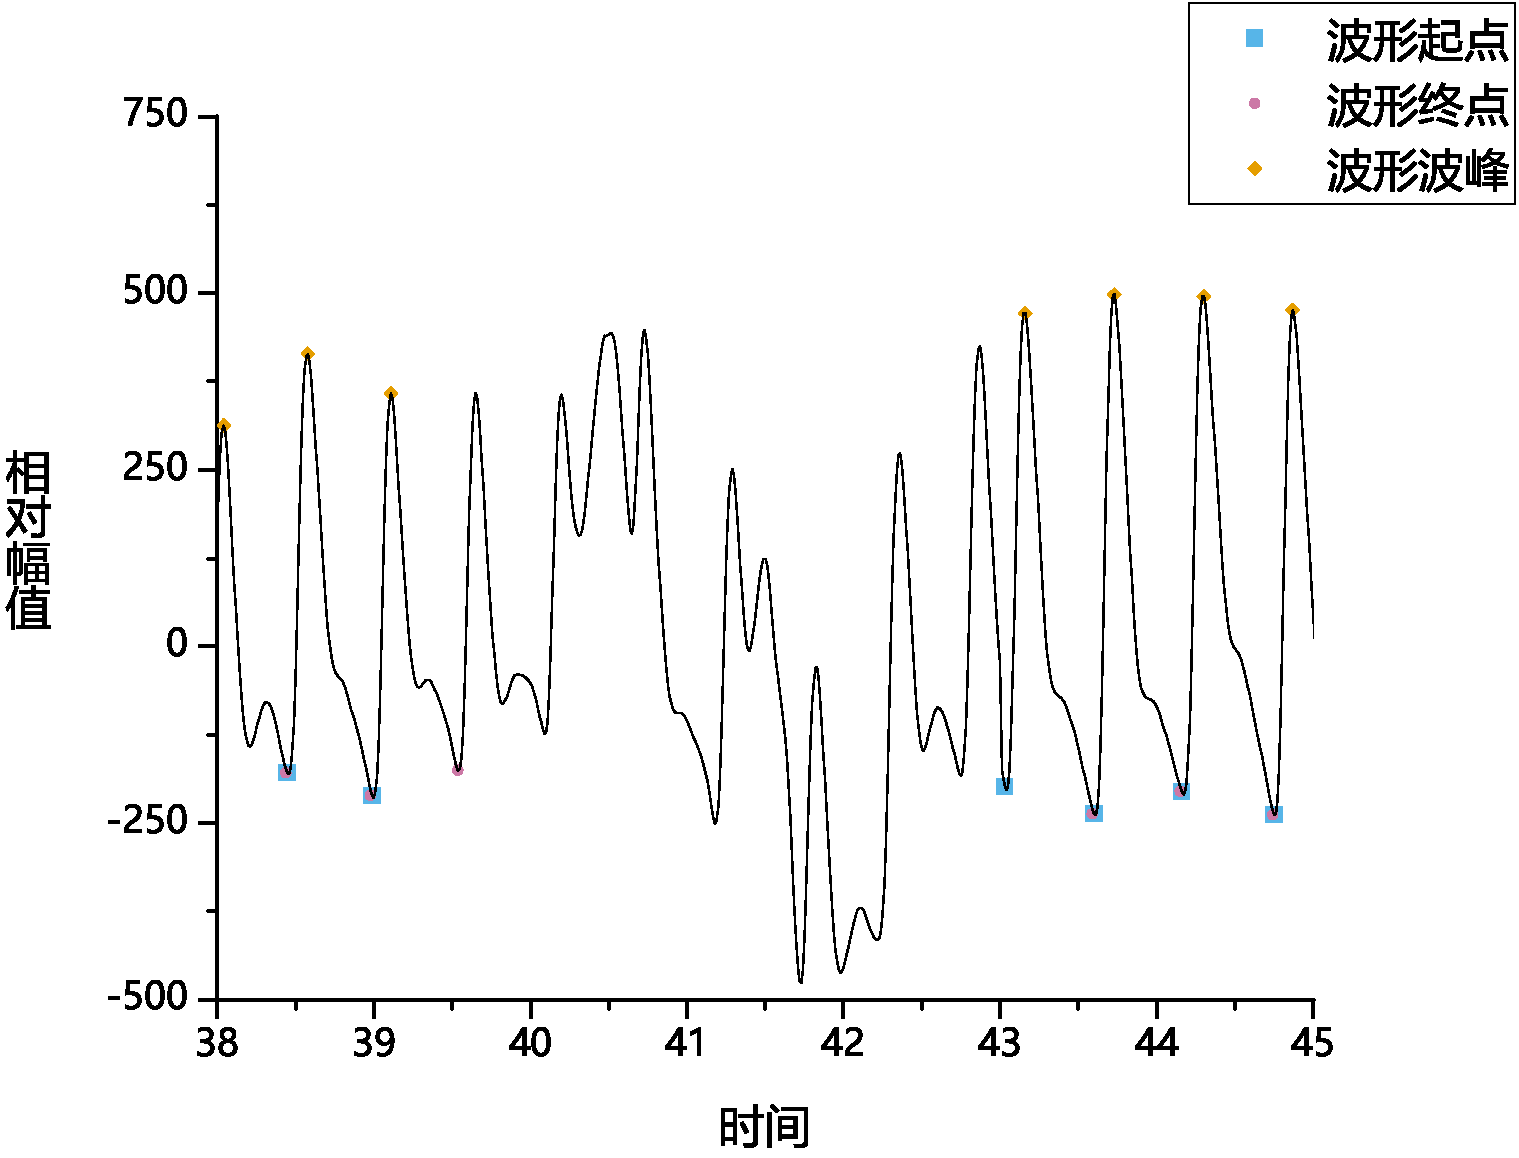
\includegraphics[width=7.5cm]{pulse_preprocess/check/why}
    }
    \quad
    \subfigure[\label{fig:c_xjh}被试XJH的波形检测结果(局部),其中6.5s处有明显错检]{
        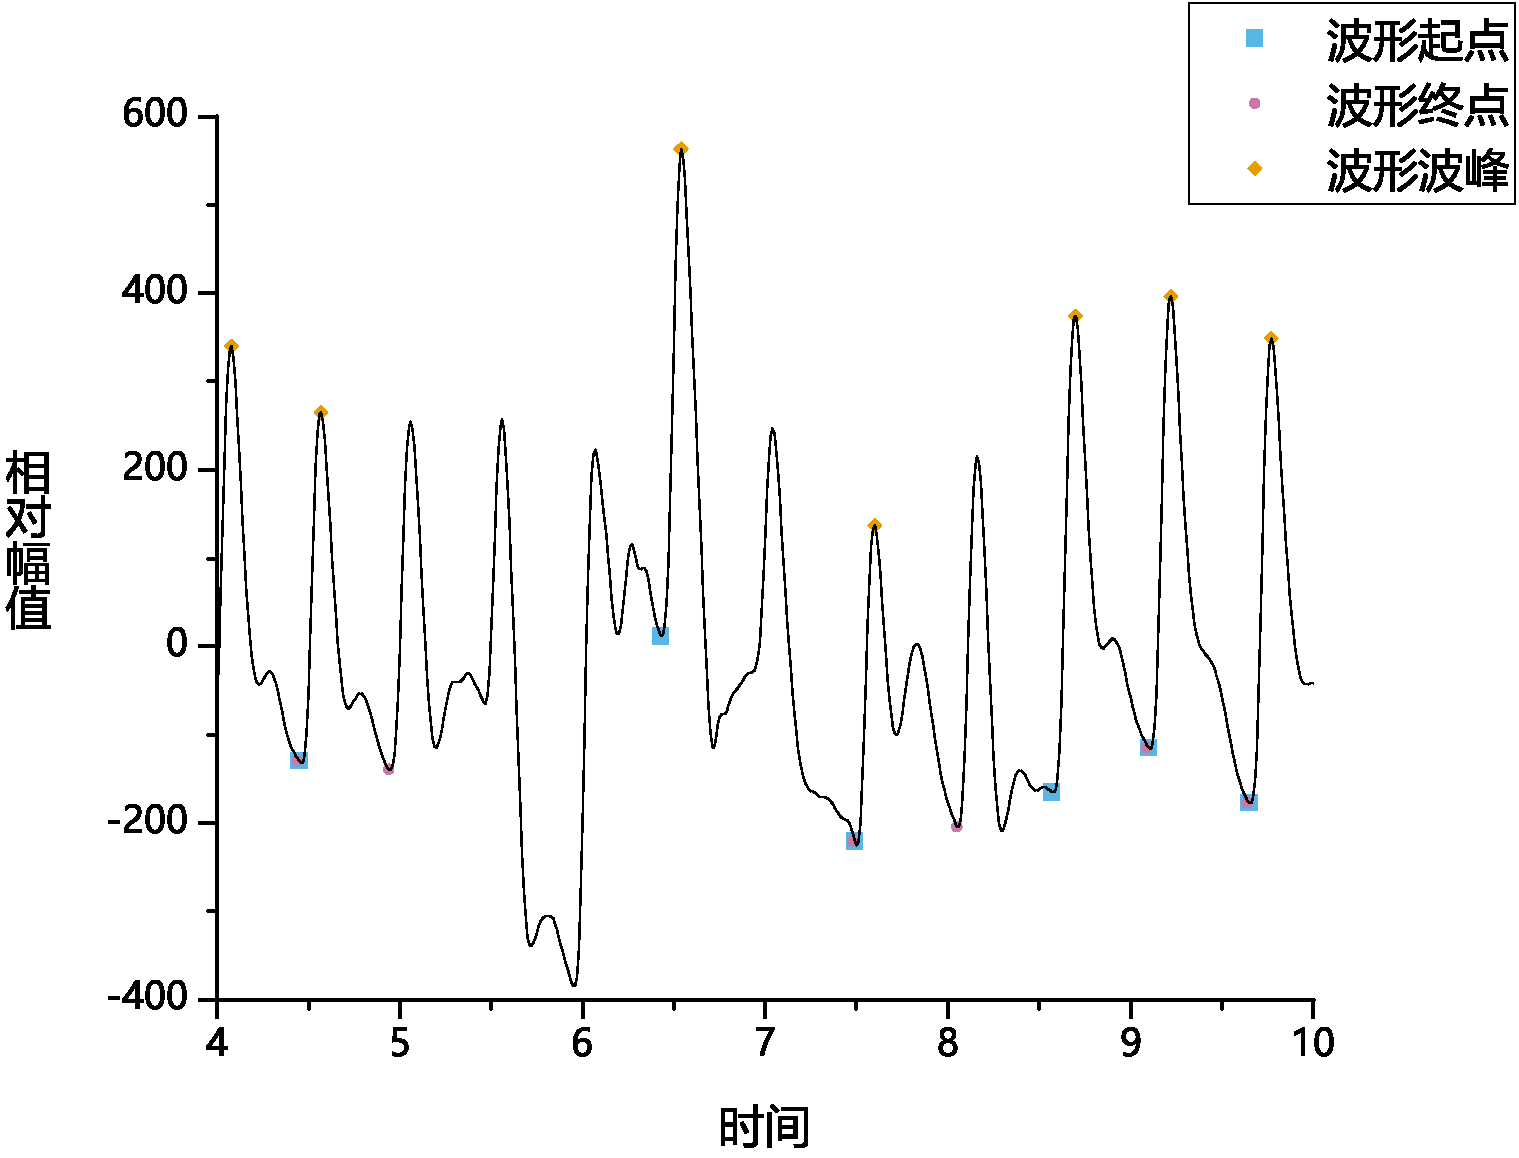
\includegraphics[width=7.5cm]{pulse_preprocess/check/xjh}
    }
    \caption[]{(续)}
\end{figure}

\section{基于SCV检测算法的一个详尽实例}

基于\autoref{fig:samplesignal}中实采信号,SCV算法对其进行波形定位检测的初筛结果如\autoref{fig:detectcheck}所示,图中波峰处数字为该波形的初筛编号。
各复核标准及最终加权投票(权值参考正文\pageref{tab:voting}页\autoref{tab:voting})的输出如\autoref{tab:detect}所示。
其中,综合标准中加粗标红的项目表示该波形可不经过加权投票直接判定为异常干扰段。
\begin{figure}[htbp]
    \centering
    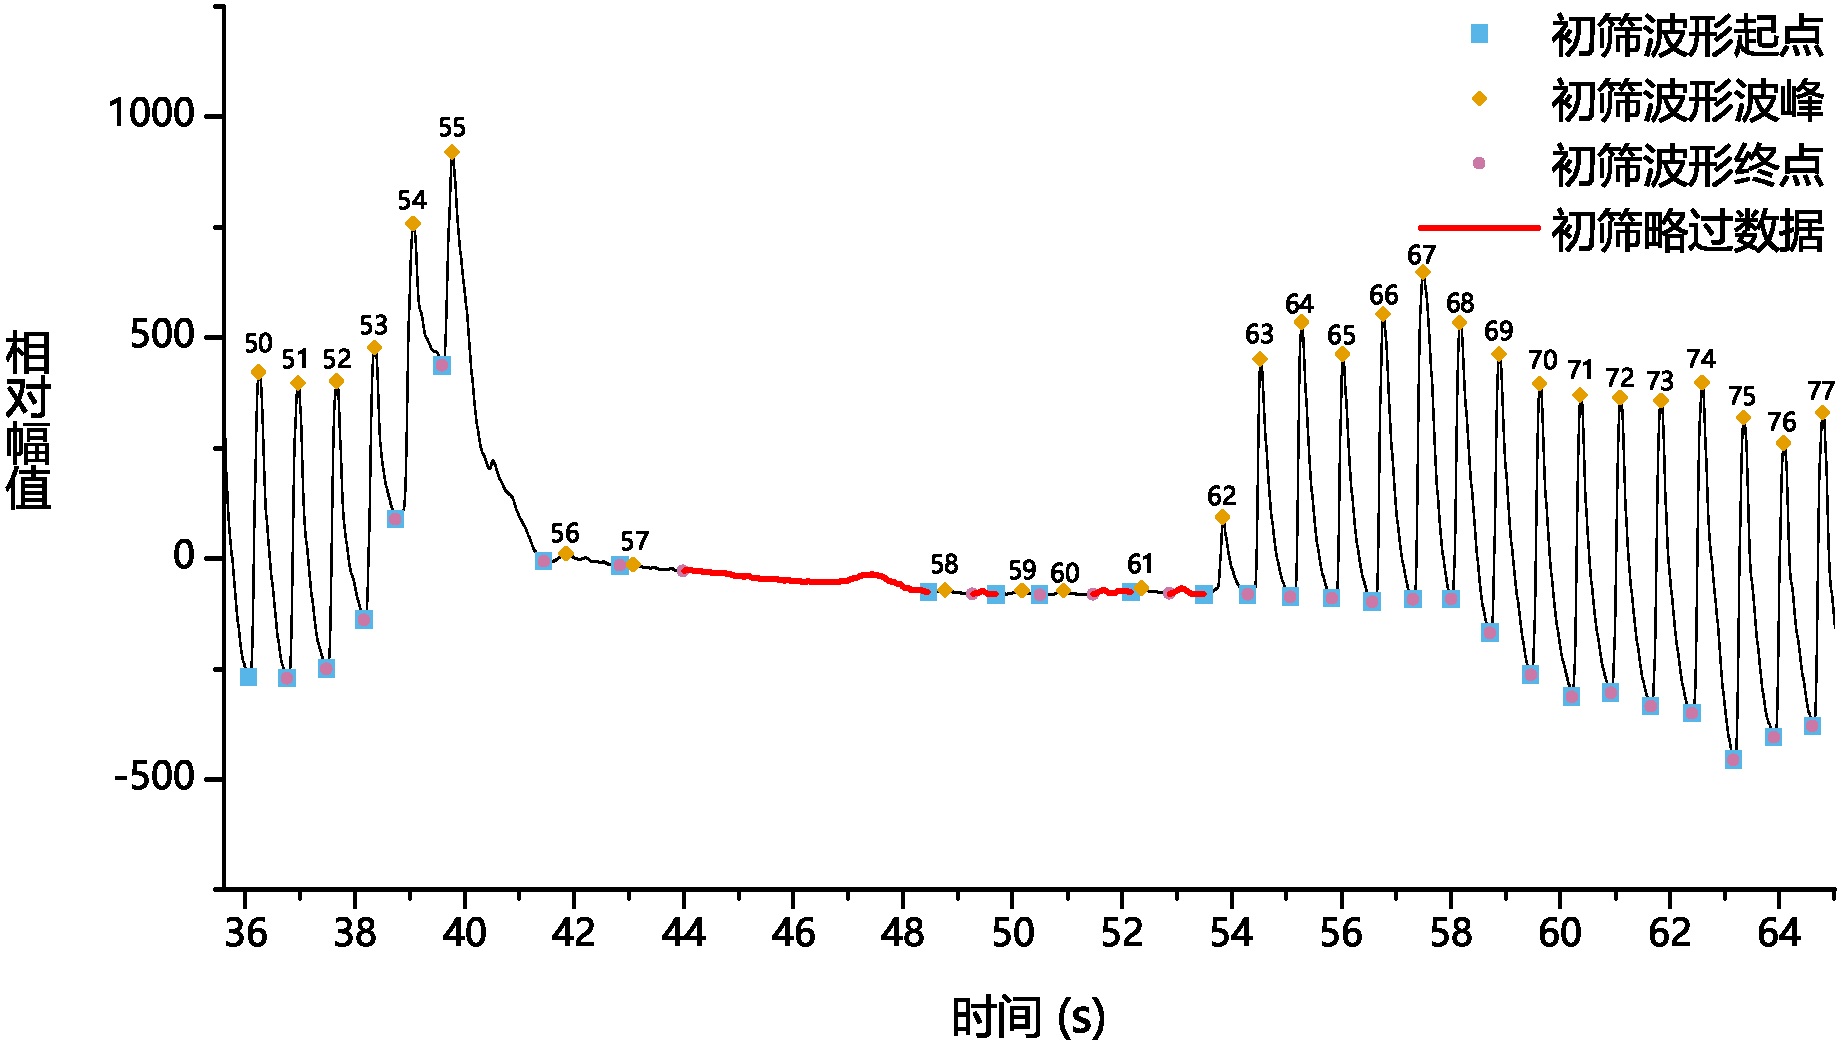
\includegraphics[width=0.9\linewidth]{pulse_preprocess/detectcheck}
    \caption{\label{fig:detectcheck}PPG波形检测算法初筛结果}
\end{figure}
\begin{landscape}
    \zihao{6}
	\begin{longtable}{m{1.5cm}<{\centering}m{1.5cm}<{\centering}m{1cm}<{\centering}m{1cm}<{\centering}m{1.5cm}<{\centering}m{1.5cm}<{\centering}m{1.5cm}<{\centering}m{2cm}<{\centering}m{2cm}<{\centering}m{2cm}<{\centering}m{2cm}<{\centering}m{1.5cm}<{\centering}}
		\caption{SCV算法对初筛波形的复核及决策输出(局部)}\\
		\label{tab:detect}\\
		\toprule
        \textbf{波形编号}&\textbf{标准差 $S$}&\textbf{能量 $P$}&\textbf{基线 $\delta B$}&\textbf{基线 $\Delta B$}&\textbf{基线 $\Delta B'$}&\textbf{时间 $PP$}&\textbf{能量类标准 $ES$}&
        \textbf{基线类标准 $ES$}&\textbf{时间类标准 $TS$}&\textbf{改良加权结果}&\textbf{最终裁决}\\
        \midrule
        \endfirsthead
        \caption[]{(续)}\\
        \midrule
        \textbf{波形编号}&\textbf{标准差 $S$}&\textbf{能量 $P$}&\textbf{基线 $\delta B$}&\textbf{基线 $\Delta B$}&\textbf{基线 $\Delta B'$}&\textbf{时间 $PP$}&\textbf{能量类标准 $ES$}&
        \textbf{基线类标准 $ES$}&\textbf{时间类标准 $TS$}&\textbf{改良加权结果}&\textbf{最终裁决}\\
        \midrule
        \endhead 
        \midrule
        \endfoot
        \bottomrule
        \endlastfoot
        …… & …… & …… & …… & …… & …… & …… & …… & …… & …… & …… & ……\\
        52 & 0 & 0 & 0 & 0 & 0 & 0 & 0 & 0 & 0 & 0 & 正常波形\\
        53 & 0 & 0 & 0 & 0 & 0 & 1 & 0 & 0 & 1 & 0.2 & 正常波形\\
        54 & 0 & 1 & 1 & 0 & 1 & 1 & 1 & \textcolor{red}{\textbf{2}}& 1 & 1 & 干扰段\\
        55 & 0 & 0 & 1 & 0 & 0 & 1 & 0 & 1 & 1 & 0.7 & 干扰段\\
        56 & 1 & 1 & 0 & 0 & 0 & 0 & \textcolor{red}{\textbf{2}}& 0 & 0 & 1 & 干扰段\\
        57 & 1 & 1 & 0 & 1 & 1 & 0 & \textcolor{red}{\textbf{2}}& \textcolor{red}{\textbf{2}}& 0 & 1 & 干扰段\\
        58 & 1 & 1 & 0 & 1 & 1 & 1 & \textcolor{red}{\textbf{2}}& \textcolor{red}{\textbf{2}}& 1 & 1 & 干扰段\\
        59 & 1 & 1 & 0 & 0 & 0 & 1 & \textcolor{red}{\textbf{2}}& 0 & 1 & 1 & 干扰段\\
        60 & 1 & 1 & 0 & 0 & 0 & 1 & \textcolor{red}{\textbf{2}}& 0 & 1 & 1 & 干扰段\\
        61 & 1 & 1 & 0 & 0 & 0 & 0 & \textcolor{red}{\textbf{2}}& 0 & 0 & 1 & 干扰段\\
        62 & 1 & 1 & 0 & 0 & 0 & 1 & \textcolor{red}{\textbf{2}}& 0 & 1 & 1 & 干扰段\\
        63 & 0 & 0 & 0 & 0 & 0 & 0 & 0 & 0 & 0 & 0 & 正常波形\\
        64 & 0 & 0 & 0 & 0 & 0 & 0 & 0 & 0 & 0 & 0 & 正常波形\\
        65 & 0 & 0 & 0 & 0 & 0 & 0 & 0 & 0 & 0 & 0 & 正常波形\\
        66 & 0 & 0 & 0 & 0 & 0 & 0 & 0 & 0 & 0 & 0 & 正常波形\\
        67 & 0 & 0 & 0 & 0 & 0 & 0 & 0 & 0 & 0 & 0 & 正常波形\\
        68 & 0 & 0 & 0 & 0 & 0 & 1 & 0 & 0 & 1 & 0.2 & 正常波形\\
        69 & 0 & 0 & 0 & 0 & 0 & 1 & 0 & 0 & 1 & 0.2 & 正常波形\\
        70 & 0 & 0 & 0 & 0 & 0 & 1 & 0 & 0 & 1 & 0.2 & 正常波形\\
        71 & 0 & 0 & 0 & 0 & 0 & 1 & 0 & 0 & 1 & 0.2 & 正常波形\\
        72 & 0 & 0 & 0 & 0 & 0 & 0 & 0 & 0 & 0 & 0 & 正常波形\\
        …… & …… & …… & …… & …… & …… & …… & …… & …… & …… & …… & ……\\
	\end{longtable}
\end{landscape}

\section{基于UCI-BP数据集的SCV算法检测详情}
使用SCV算法对UCI-BP数据集\path{Part_1.mat}文件的前50条数据记录进行了分析,统计详情如\autoref{tab:ucibp_details}所示。
此外,\autoref{fig:ucibp_detect_details}也给出了基于UCI-BP数据集的展现SCV算法优异的检测性能的一些典型案例。
\begin{center}
    \zihao{5}
    \begin{longtable}{m{1.5cm}<{\centering}m{1.5cm}<{\centering}m{1.5cm}<{\centering}m{1.5cm}<{\centering}m{1.5cm}<{\centering}m{1.5cm}<{\centering}m{1.5cm}<{\centering}m{1.5cm}<{\centering}} 
        \caption{基于UCI-BP数据库的SCV算法检测效果统计}\\
		\label{tab:ucibp_details}\\
        \toprule
        \textbf{编号} & \textbf{检测总数} & \textbf{错检数} & \textbf{正确率} & \textbf{编号} & \textbf{检测总数} & \textbf{错检数} & \textbf{正确率}  \\
        \midrule
        \endfirsthead
        \caption[]{(续)}\\
        \toprule
        \textbf{编号} & \textbf{检测总数} & \textbf{错检数} & \textbf{正确率} & \textbf{编号} & \textbf{检测总数} & \textbf{错检数} & \textbf{正确率}  \\
        \midrule
        \endhead 
        \bottomrule
        \endfoot
        \bottomrule
        \endlastfoot
        1	&   960 	&8	    &99.17\%	    &26	    &   48	 &0	    &100.00\%   \\
        2	&   931 	&5	    &99.46\%	    &27	    &   48	 &0	    &100.00\%   \\
        3	&   718 	&2	    &99.72\%	    &28	    &   59	 &1	    &98.31\%    \\    
        4	&   1062	&0	    &100.00\% 	    &29     &	72   &0     &100.00\%   \\
        5	&   976 	&2	    &99.80\%	    &30	    &   72	 &0	    &100.00\%   \\
        6	&   301 	&1	    &99.67\%	    &31	    &   59	 &0	    &100.00\%   \\
        7	&   1021	&3	    &99.71\%	    &32	    &   34	 &0	    &100.00\%   \\
        8	&   55	    &0	    &100.00\% 	    &33     &	60   &0     &100.00\%   \\
        9	&   26	    &0	    &100.00\% 	    &34     &	72   &0     &100.00\%   \\
        10	&   10	    &0	    &100.00\% 	    &35     &	73   &0     &100.00\%   \\
        11	&   9       &0      &100.00\%       &36	    &   926  &0	    &100.00\%   \\
        12	&   26	    &0	    &100.00\% 	    &37     &	913  &0	    &100.00\%   \\
        13	&   12	    &0	    &100.00\% 	    &38     &	607  &0 	&100.00\%   \\
        14	&   12	    &0	    &100.00\% 	    &39     &	199  &0	    &100.00\%   \\
        15	&   402 	&2	    &99.50\%	    &40	    &   755  &0     &100.00\%   \\
        16	&   957 	&10 	&98.96\%  	    &41     &	902  &0	    &100.00\%   \\
        17	&   891 	&3	    &99.66\%	    &42	    &   912  &0     &100.00\%   \\
        18	&   314 	&5	    &98.41\%	    &43	    &   135  &0     &100.00\%   \\
        19	&   802 	&5	    &99.38\%	    &44	    &   22	 &0	    &100.00\%   \\
        20	&   19	    &0	    &100.00\% 	    &45     &	72   &0     &100.00\%   \\
        21	&   19	    &0	    &100.00\% 	    &46     &	83   &0     &100.00\%   \\
        22	&   9	    &0      &100.0 0\%	    &47	    &   846  &1	    &99.88\%    \\
        23	&   44	    &0	    &100.00\% 	    &48     &	9	 &0	    &100.00\%   \\
        24	&   59	    &0	    &100.00\% 	    &49     &	44   &1     &97.73\%    \\
        25	&   897 	&1	    &99.89\%	    &50	    &   8	 &0     &100.00\%   \\
        合计&           &       &               &       &   17562&50    &99.72\%    \\
	\end{longtable}
\end{center}
\begin{figure}[htbp]
    \centering
    \subfigure[\label{fig:c_0003}数据编号0003的波形检测结果(局部)]{
    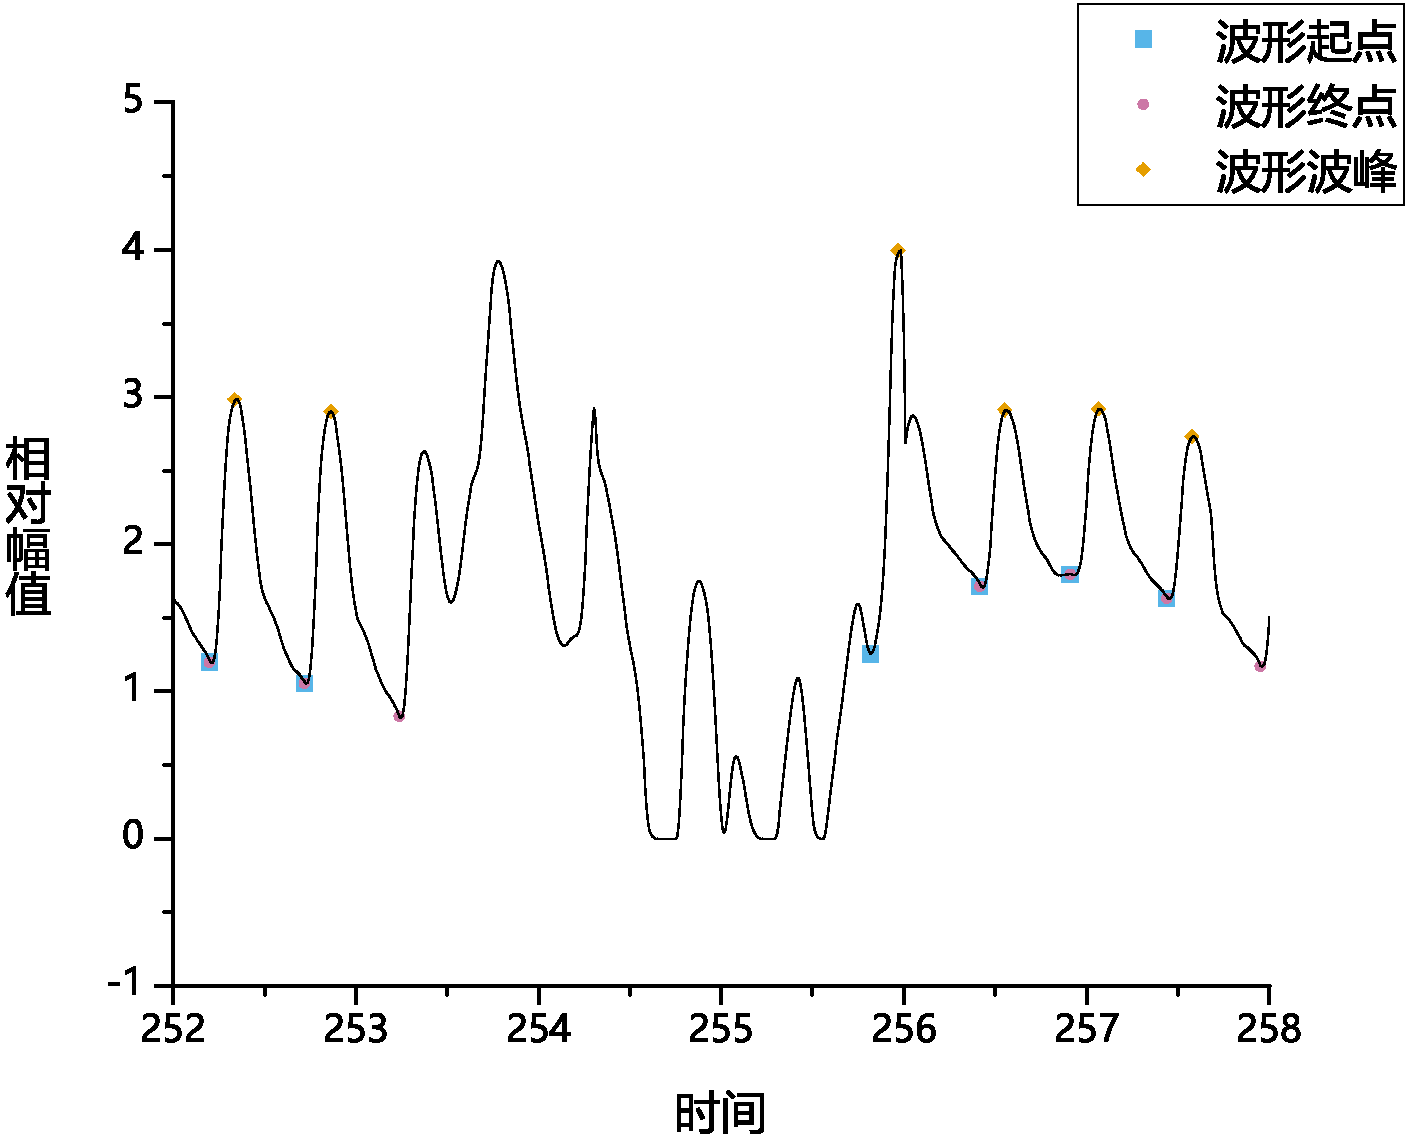
\includegraphics[width=7.5cm]{pulse_preprocess/check/0003}
    }
    \quad
    \subfigure[\label{fig:c_0016}数据编号0016的波形检测结果(局部)]{
    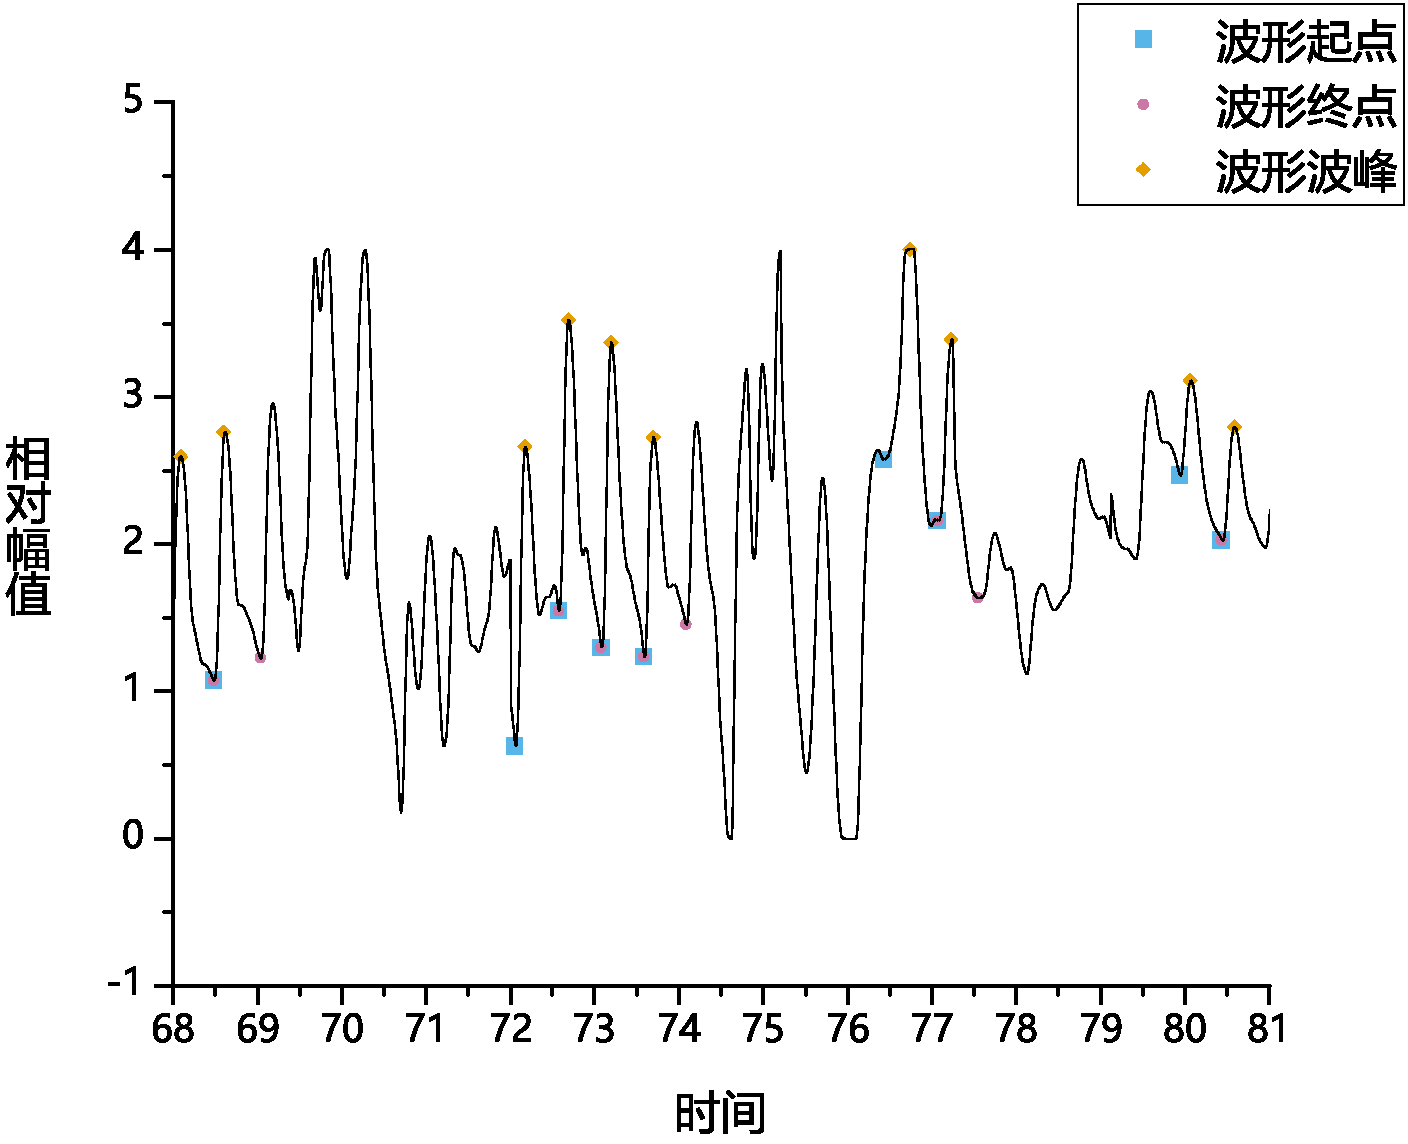
\includegraphics[width=7.5cm]{pulse_preprocess/check/0016}
    }
    \quad
    \subfigure[\label{fig:c_0017}数据编号0017的波形检测结果(局部)]{
        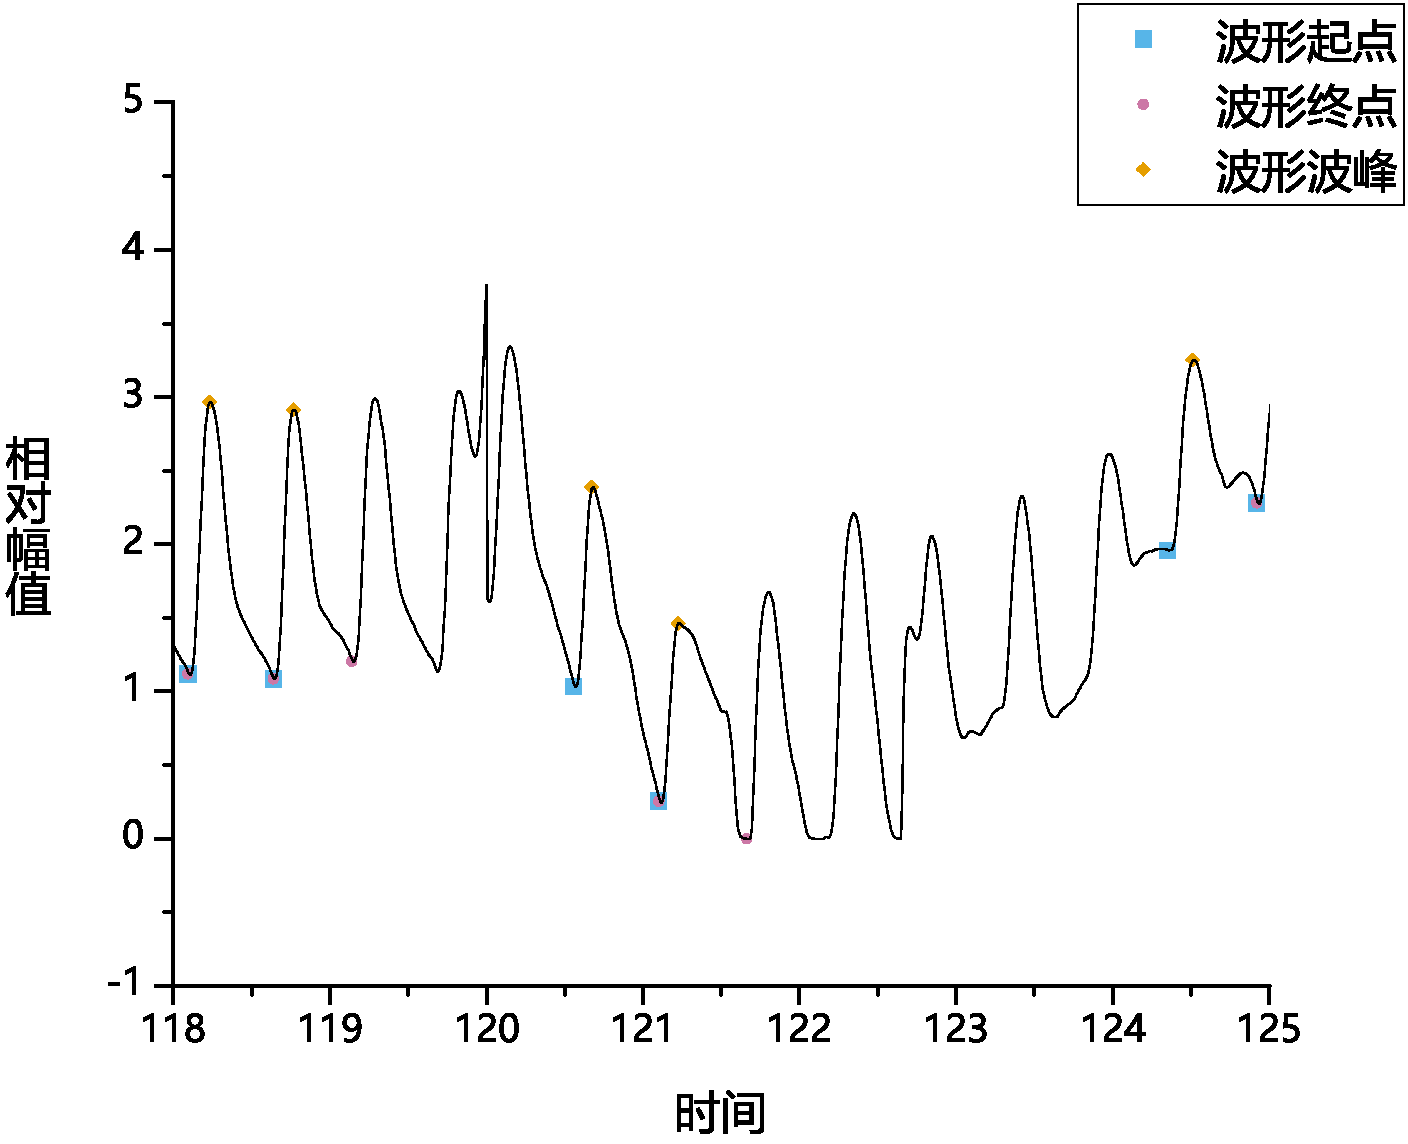
\includegraphics[width=7.5cm]{pulse_preprocess/check/0017}
    }
    \quad
    \subfigure[\label{fig:c_0019}数据编号0019的波形检测结果(局部),其中126s与129s处有明显错检]{
        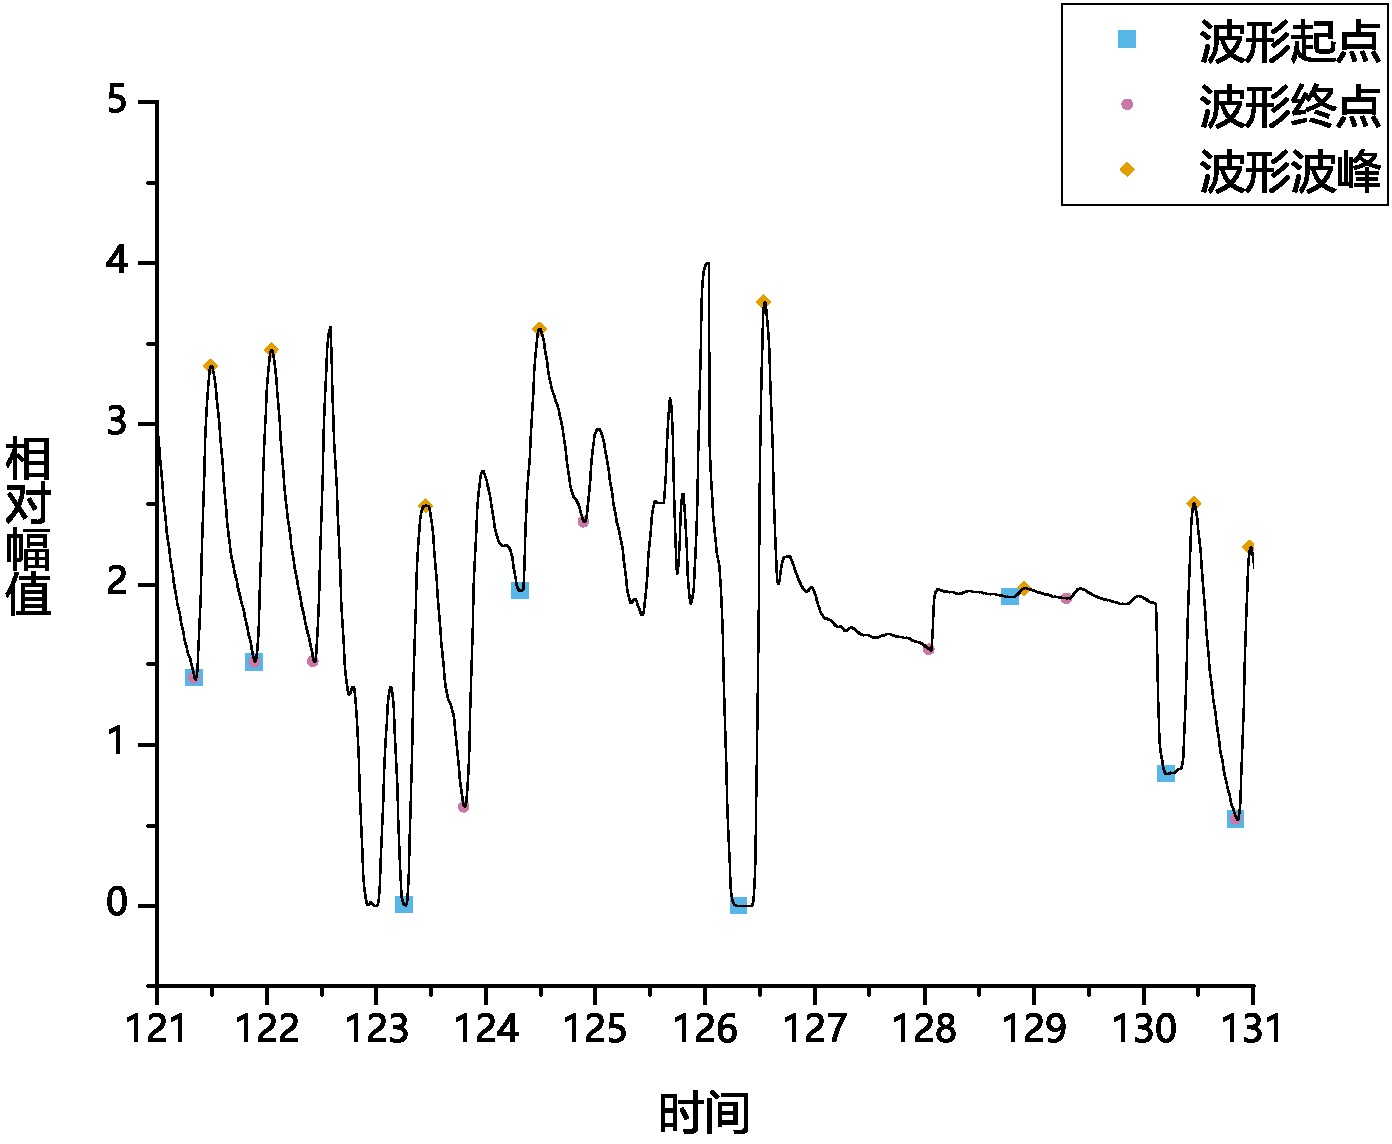
\includegraphics[width=7.5cm]{pulse_preprocess/check/0019}
    }
    \caption{\label{fig:ucibp_detect_details}SCV算法对UCI-BP数据集中复杂信号的检测效果示意}
\end{figure}

\section{机器学习领域的专业术语简表}
参见
\begin{center}
    \begin{longtable}{m{3cm}m{5cm}m{7cm}}
        \toprule
        \textbf{中文全称}&\textbf{英文全称}&\textbf{含义}\\
        \midrule
        \endfirsthead
        \toprule
        \textbf{中文全称}&\textbf{英文全称}&\textbf{含义}\\
        \midrule
        \endhead 
        \bottomrule
        \endfoot
        \bottomrule
        \endlastfoot
        模型        &   model               &   计算机层面的认知        \\
        学习算法    &   learning algorithm  &   从数据中产生模型的方法  \\
        数据集      &   data set            &    一组记录的合集         \\
        示例        &   instance            &   对于某个对象的描述      \\
        样本        &   sample              &   也叫示例                \\
        属性        &   attribute           &   对象的某方面表现或特征  \\
        特征        &   feature             &   同属性                  \\
        属性值      &   attribute value     &   属性上的取值            \\
        属性空间    &   attribute space     &   属性张成的空间          \\
        样本空间    &   sample space        &   同属性空间              \\
        特征向量    &   feature vector      &   在属性空间里每个点对应一个坐标向量,把一个示例称作特征向量\\
        维数        &   dimensionality      &   描述样本参数的个数(也就是空间是几维的)\\
        学习        &   learning            &   从数据中学得模型        \\
        训练        &   training            &   同学习                  \\
        训练数据    &   training data       &   训练过程中用到的数据    \\
        训练样本    &   training sample     &   训练用到的每个样本      \\
        训练集      &   training set        &   训练样本组成的集合      \\
        假设        &   hypothesis          &   学习模型对应了关于数据的某种潜在规则\\
        真相        &   ground-truth        &   真正存在的潜在规律      \\
        学习器      &   learner             &   模型的另一种叫法,把学习算法在给定数据和参数空间的实例化\\
        预测        &   prediction          &   判断一个东西的属性      \\
        标记        &   label               &   关于示例的结果信息      \\
        样例        &   example             &   拥有标记的示例          \\
        标记空间    &   label space         &   所有标记的集合          \\
        分类        &   classification      &   预测是离散值            \\
        回归        &   regression          &   预测值是连续值          \\
        二分类      &   binary classification   &   只涉及两个类别的分类任务    \\
        正类        &   positive class      &   二分类里的一个          \\
        反类        &   negative class      &   二分类里的另外一个          \\
        多分类      &   multi-class classification  &   涉及多个类别的分类  \\
        测试        &   testing             &   学习到模型之后对样本进行预测的过程  \\
        测试样本    &   testing sample      &   被预测的样本    \\
        聚类        &   clustering          &   把训练集中的对象分为若干组  \\
        簇          &   cluster             &   每一个组叫簇            \\
        监督学习    &   supervised learning  &   典范:分类和回归       \\
        无监督学习  &   unsupervised learning  &    典范--聚类          \\
        未见示例    &   unseen instance       &   “新样本”,没训练过的样本    \\
        泛化        &   generalization          &   学得的模型适用于新样本的能力    \\
        分布        &   distribution        &   样本空间的全体样本服从的一种规律\\
        独立同分布  &   independent and identically distributed &   获得的每个样本都是独立地从这个分布上采样获得的  \\
	\end{longtable}
\end{center}

\section{本研究所使用的软件及工程项目}
在本文研究及论文写作过程中,
开发软件及工具

\section{批处理操作及参数设置说明}
一、目的

保存当前对PPG读取分析的相关操作,供下次调用快速使用。典型的应用场景为,调整了脉搏波的输出特征后,需要对所有数据进行新一轮的分析,此时脉搏波的定位结果可以完全沿用上一轮分析结果。若上一轮分析结果已被保存,则当前新一轮分析即可批量处理完成。

二、操作流程

1. 设置需要批处理的目录

批处理是以目录为单位进行。通过批处理->生成模板,选择目录后,即可在该目录下生成空白的配置文件。

2. 手动调整配置文件的相关参数

默认的配置文件具有的功能有限。需要根据具体数据灵活调整,由于一般数据文件在整个分析周期内是固定不变的。因此,配置文件设置完成后(特别是对脉搏波波形的取舍设置),可以在整个分析周期内通用。

3. 选择设置好的配置文件完成批处理

通过软件选择批处理->开始批处理,选择相应的配置文件,按配置完成批处理过程。

三、参数配置说明

1. 语法

配置文件必须是合法的Json文件。

2. 字段说明

\Rnum{1}. path 

当前需要批处理的目录。无需手动调整。

\Rnum{2}. PEstate

当前目录下所有数据的PE状态,值域[0,1]。需要手动设置。

\Rnum{3}. mode

当前批处理所需要进行的批处理操作,可自定义设置。目前支持打开文件、算法初步确认、人工手动调整检测结果、导出检测结果、开始特征分析、导出分析特征及分析结果上传等7种操作。其中,后6种文件操作在批处理过程中统一配置。分别通过mode的1位来完成控制。算法初步确认对应mode的最低位。mode的默认值为31,即0b011111,即对当前目录下所有数据文件进行出数据特征上传外的所有操作。
需要注意的是,可配置的6个操作有着逻辑上的依赖关系,某些配置可能会导致程序无法运行。如出现此种情况,请联系作者。

\Rnum{4}. files

当前批处理操作所需处理的所有数据文件项。批处理会依次对file中所有数据项进行处理。需要对其中的一定数据项进行自定义配置。

\Rnum{5}. path in files

需要处理的数据文件名。默认生成,无需修改。

\Rnum{6}. skipped in files

是否跳过处理该数据文件,可自定义配置。默认为false,即不跳过。

\Rnum{7}. pulses in files

对该数据波形自动分析结果得到的脉搏波波形的删除或新增操作,可自定义配置。默认为空,即接受算法全部处理结果。若需要配置,需要新增一个包含type与points两个字段的Json数据项至pulses。可根据需要配置多个这样的数据项。

\Rnum{8}. type in pulses in files

指定对脉搏波波形操作类型,必须配置。可选字段,A与R。前者对应新增(add),后者对应删除(remove)。目前不接受其他字段。

\Rnum{9}. Points in pulses in files

定义需要新增或移除的脉搏波的坐标位置,必须是三元数组(对应起点、峰值点及终点),必须配置。其中,峰值点数值决定了当前波形的新增或移除是否成功。新增波形时,三者的数值准确性要求较低,可允许10以内的误差。移除时,必须保证坐标位置的准确性。

四、配置范例及说明

\lstinputlisting[caption={配置范例},label=lst:json_conf,style=myJava]{code/appendix/demo.json}

上述配置文件可对\path{D:/UrgeData/Documents/ppgdata/No}文件夹下的\path{by_wavePLETH_2017080113.csv}等文件进行批处理。其中,PEstate被设置为0,表示当前目录下全为健康人群数据文件。
mode被配置为31,所有文件会完成算法初步确认、人工手动调整检测结果、导出检测结果、开始特征分析、导出分析特征等操作。在对\path{by_wavePLETH_2017080113.csv}文件处理时,
不需跳过处理,对算法的自动检测结果需先移除$(91,105,177)$处的脉搏波波形,再在$(91,105,177)$处新增一个脉搏波波形。
}